% Original TikZ/PGF schematic created for the revised Helmholtz/PML manuscript.
% This is a new construction from finite-volume geometry, not a traced image.
% License: CC-BY-4.0; https://creativecommons.org/licenses/by/4.0/
% Input inside a figure environment; requires the tikz package.
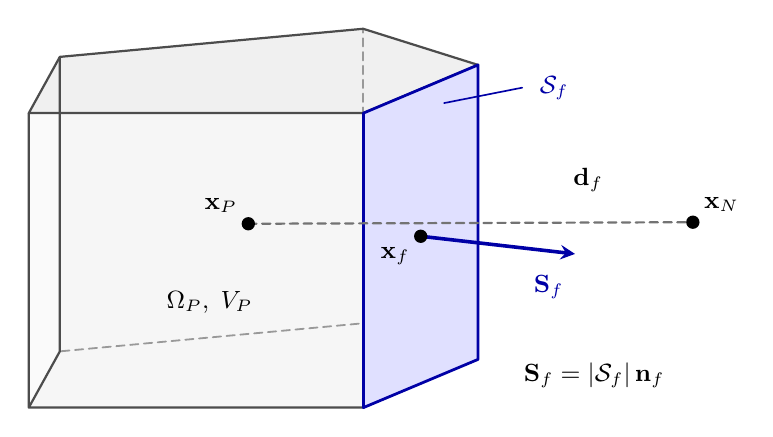
\begin{tikzpicture}[
    x={(1.7cm,0cm)}, y={(0.646cm,0.51cm)}, z={(0cm,1.7cm)},
    line join=round, line cap=round, >=stealth,
    every node/.style={font=\small},
    edge/.style={draw=black!70,line width=0.8pt},
    hidden/.style={draw=black!40,densely dashed,line width=0.65pt},
    centre/.style={circle,fill=black,inner sep=1.7pt}
]
    % A pentagonal prism is a polyhedral control volume.  Its shared face
    % joins (2.5,0,z) and (2.9,1.2,z); its outward normal is (1.2,-0.4,0).
    \coordinate (A) at (0,0,0);
    \coordinate (B) at (2.5,0,0);
    \coordinate (C) at (2.9,1.2,0);
    \coordinate (D) at (1.7,2.1,0);
    \coordinate (E) at (-0.3,1.4,0);
    \coordinate (At) at (0,0,2.2);
    \coordinate (Bt) at (2.5,0,2.2);
    \coordinate (Ct) at (2.9,1.2,2.2);
    \coordinate (Dt) at (1.7,2.1,2.2);
    \coordinate (Et) at (-0.3,1.4,2.2);

    % Light faces and dashed rear edges keep the cell centre visible.
    \fill[gray!7] (A)--(B)--(Bt)--(At)--cycle;
    \fill[gray!4] (E)--(A)--(At)--(Et)--cycle;
    \fill[gray!12] (At)--(Bt)--(Ct)--(Dt)--(Et)--cycle;
    \draw[hidden] (B)--(C)--(D)--(E);
    \draw[hidden] (C)--(Ct) (D)--(Dt);
    \draw[edge] (E)--(A)--(B) (E)--(Et) (A)--(At) (B)--(Bt);
    \draw[edge] (At)--(Bt)--(Ct)--(Dt)--(Et)--cycle;

    % Highlight the common face, without implying any phase partition.
    \path[fill=blue!12,draw=blue!65!black,line width=1.0pt]
        (B)--(C)--(Ct)--(Bt)--cycle;

    \coordinate (P) at (1.2937044400,0.9111994698,1.1);
    \coordinate (F) at (2.7,0.6,1.1);
    \coordinate (N) at (4.6,0.95,1.1);
    \coordinate (S) at (4.02,0.16,1.1);

    \draw[black!55,densely dashed,line width=0.8pt] (P)--(N);
    \node[fill=white,inner sep=1pt] at (3.8,1.0,1.40)
        {$\mathbf d_f$};
    \draw[->,blue!65!black,line width=1.3pt] (F)--(S)
        node[pos=0.83,below=5pt] {$\mathbf S_f$};

    \node[centre,label={[inner sep=2pt]above left:$\mathbf x_P$}] at (P) {};
    \node[centre,label={[inner sep=2pt]below left:$\mathbf x_f$}] at (F) {};
    \node[centre,label={[inner sep=2pt]above right:$\mathbf x_N$}] at (N) {};
    \node[fill=gray!7,inner sep=1.5pt] at (1.18,0.45,0.65) {$\Omega_P,\;V_P$};
    \node[anchor=west,text=blue!65!black] at (3.48,0.7,2.18)
        {$\mathcal S_f$};
    \draw[blue!65!black,line width=0.6pt]
        (3.42,0.7,2.18)--(2.78,0.85,2.02);

    \node[anchor=west] at (3.55,0.2,0.18)
        {$\mathbf S_f=|\mathcal S_f|\,\mathbf n_f$};
\end{tikzpicture}
